% Ensure that you compile using XeLaTeX !!! PDFTex has problems with some of the packages used
\documentclass[12pt]{article}
\setlength\parindent{0pt}

\usepackage{parskip}
\usepackage[margin=0.5in]{geometry}
\usepackage{fullpage}
\usepackage{moresize}
\usepackage{graphicx}
\usepackage{caption}
\usepackage{subcaption}
\usepackage{float}
\usepackage{xcolor}
\usepackage{soul}
\usepackage{fontspec}
\setmainfont{Doulos SIL}

\begin{document}

\begin{center}
\textbf{{\color{violet}{\HUGE 20201007 Wednesday\\}}}

\textbf{{\color{violet}{\HUGE ALL EXAMS\\}}}

\end{center}
\newpage

\begin{center}
\textbf{{\color{blue}{\HUGE START OF EXAM\\}}}

\textbf{{\color{blue}{\HUGE Student ID: 23100\\}}}

\textbf{{\color{blue}{\HUGE 9:00\\}}}

\end{center}
\newpage

{\large Question 1}\\

Topic: Phonological Features\\
Source: Week 4 Discussion\\

Explain why the given feature's value varies across this set of sounds.\\

{[sonorant]}

alveolars


\newpage

{\large Question 2}\\

Topic: Articulatory Phonetics\\
Source: Week 2 Discussion\\

Explain why it's possible to say that signed languages have articulatory phonetics.\\


\newpage

\begin{center}
\textbf{{\color{red}{\HUGE END OF EXAM}}}\\

\end{center}
\newpage

\begin{center}
\textbf{{\color{blue}{\HUGE START OF EXAM\\}}}

\textbf{{\color{blue}{\HUGE Student ID: 23000\\}}}

\textbf{{\color{blue}{\HUGE 9:10\\}}}

\end{center}
\newpage

{\large Question 1}\\

Topic: Other (pre-midterm)\\
Source: Week 4 Handout, Part II, Question 2(iv)\\

Explain how you would figure out the Swahili word for this English gloss.\\

‘I wanted them.’

\begin{figure}[H]
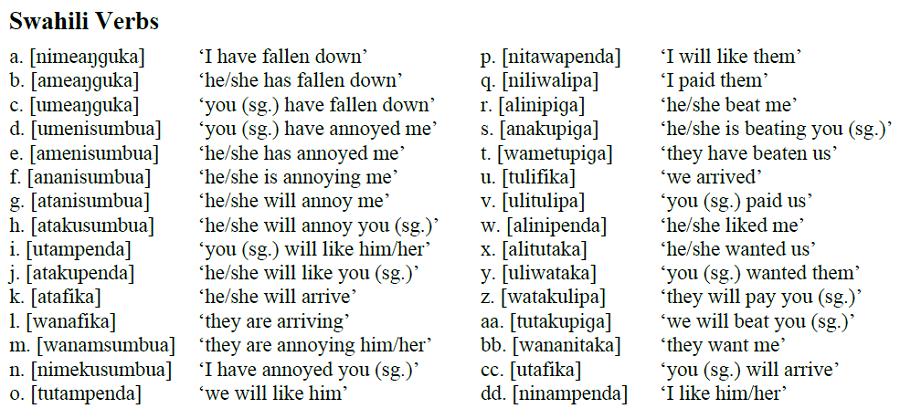
\includegraphics{../images/swahiliverbs.png}
\end{figure}

\newpage

{\large Question 2}\\

Topic: Phonological Features\\
Source: Week 4 Discussion\\

Explain why phonological features are used instead of phonetic characteristics in analyzing datasets.\\


\newpage

\begin{center}
\textbf{{\color{red}{\HUGE END OF EXAM}}}\\

\end{center}
\newpage

\begin{center}
\textbf{{\color{blue}{\HUGE START OF EXAM\\}}}

\textbf{{\color{blue}{\HUGE Student ID: 23000\\}}}

\textbf{{\color{blue}{\HUGE 9:20\\}}}

\end{center}
\newpage

{\large Question 1}\\

Topic: Other (pre-midterm)\\
Source: Week 4 Handout, Part II, Question 2(iv)\\

Explain how you would figure out the Swahili word for this English gloss.\\

‘I wanted them.’

\begin{figure}[H]
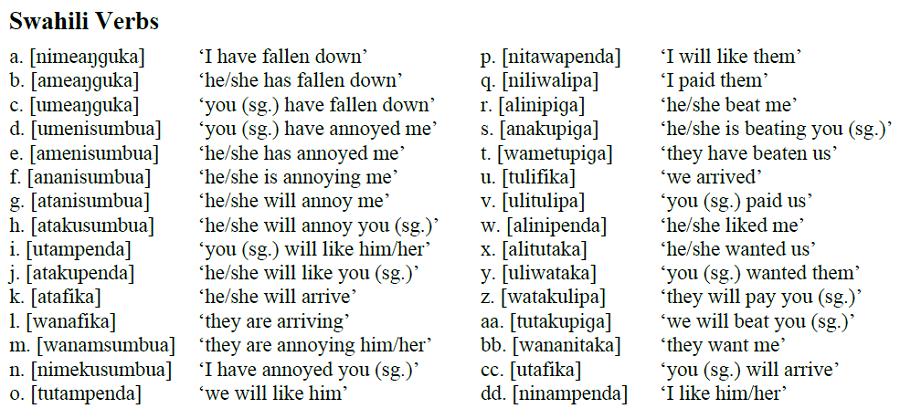
\includegraphics{../images/swahiliverbs.png}
\end{figure}

\newpage

{\large Question 2}\\

Topic: Phonological Features\\
Source: Week 4 Discussion\\

Explain why phonological features are used instead of phonetic characteristics in analyzing datasets.\\


\newpage

\begin{center}
\textbf{{\color{red}{\HUGE END OF EXAM}}}\\

\end{center}
\newpage

\begin{center}
\textbf{{\color{blue}{\HUGE START OF EXAM\\}}}

\textbf{{\color{blue}{\HUGE Student ID: 51697\\}}}

\textbf{{\color{blue}{\HUGE 9:30\\}}}

\end{center}
\newpage

{\large Question 1}\\

Topic: Other (pre-midterm)\\
Source: Week 4 Handout, Part II, Question 3\\

Explain how you would figure out what the Luiseño form is for the morpheme whose meaning is given below.\\

‘make / cause’

\begin{figure}[H]
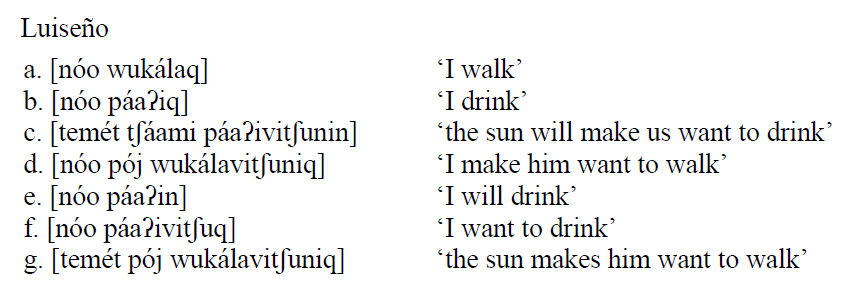
\includegraphics{../images/luiseno.png}
\end{figure}

\newpage

{\large Question 2}\\

Topic: Phonological Features\\
Source: Week 4 Discussion\\

Explain why phonological features are used instead of phonetic characteristics in analyzing datasets.\\


\newpage

\begin{center}
\textbf{{\color{red}{\HUGE END OF EXAM}}}\\

\end{center}
\newpage

\begin{center}
\textbf{{\color{blue}{\HUGE START OF EXAM\\}}}

\textbf{{\color{blue}{\HUGE Student ID: 16758\\}}}

\textbf{{\color{blue}{\HUGE 9:40\\}}}

\end{center}
\newpage

{\large Question 1}\\

Topic: Other (pre-midterm)\\
Source: Week 4 Handout, Part II, Question 3\\

Explain how you would figure out what the Luiseño form is for the morpheme whose meaning is given below.\\

‘first person plural object’ (‘us’)

\begin{figure}[H]
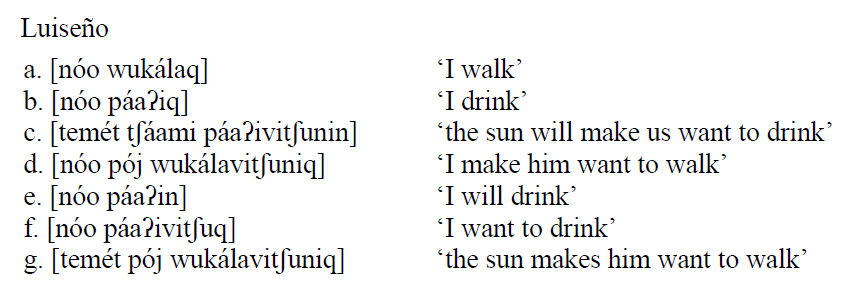
\includegraphics{../images/luiseno.png}
\end{figure}

\newpage

{\large Question 2}\\

Topic: Transcription\\
Source: Week 2 Handout, Part II\\

Is this a reasonable transcription of this word? Explain why.\\

<choose>: {[t͡ʃuz]}


\newpage

\begin{center}
\textbf{{\color{red}{\HUGE END OF EXAM}}}\\

\end{center}
\newpage

\begin{center}
\textbf{{\color{blue}{\HUGE START OF EXAM\\}}}

\textbf{{\color{blue}{\HUGE Student ID: 12991\\}}}

\textbf{{\color{blue}{\HUGE 9:50\\}}}

\end{center}
\newpage

{\large Question 1}\\

Topic: Other (pre-midterm)\\
Source: Week 2 Handout, Part I, Question 8\\

Is this question about phonetics or phonology, and why? (To be clear: you do NOT need to answer the question itself -- just tell me whether it's a question about phonetics or phonology.)\\

Consider the following two words from American Sign Language. The first one means LUCKY, while the second means SMART. How would you describe the difference between the ``pronunciation'' (articulation) of these two words? Note that in each case, the image to the left is the starting position of the sign, while the one to the right is the ending position.

\begin{figure}[H]
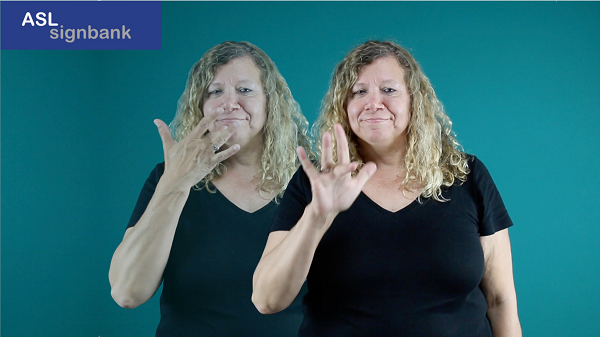
\includegraphics{../images/asl_lucky.png}
\end{figure}
\begin{figure}[H]
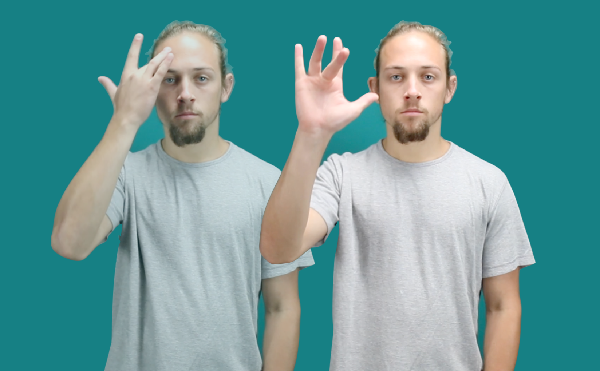
\includegraphics{../images/asl_smart.png}
\end{figure}

\newpage

{\large Question 2}\\

Topic: Phonological Features\\
Source: Week 4 Discussion\\

Explain why phonological features are used instead of phonetic characteristics in analyzing datasets.\\


\newpage

\begin{center}
\textbf{{\color{red}{\HUGE END OF EXAM}}}\\

\end{center}
\newpage

\end{document}

